\documentclass{article}
\usepackage{geometry}
\geometry{a4paper, margin=1in}
\usepackage{graphicx}
\usepackage{listings}
\usepackage{xcolor}
\usepackage[utf8]{inputenc}

\lstset{
    basicstyle=\ttfamily\small,
    breaklines=true,
    frame=single,
    language=C++,
    keywordstyle=\color{blue},
    commentstyle=\color{green!50!black},
    stringstyle=\color{red},
    showstringspaces=false
}

\begin{document}

\title{Operating Systems Lab Assignment: Thread-Safe Data Structures}
\author{Your Name}
\date{November 17, 2026}
\maketitle

\section{Introduction}
This lab was about making data structures thread safe in C++ using mutexes. I did the queue and stack for exercise 1 and then the priority queue, circular buffer, deque and linked list. Everything compiled with g++ using -pthread and -std=c++11 and ran fine.

\section{Exercise 1: Thread-Safe Queue and Stack}
\lstinputlisting[language=C++]{thread_safe_data_structures.cpp}

Each class has a mutex and every function uses lock\_guard to lock it. lock\_guard unlocks by itself when the function ends so you dont have to call unlock. Pop checks empty, gets the value and removes it all under one lock so two threads cant pop the same thing.

In the producer consumer part 3 producers push 5 messages each (15 total) and 2 consumers pop them. messages\_produced is atomic so the count stays right. The consumers stop when all 15 are produced and the queue is empty. In my output all 15 messages got processed. The order is different every time because of how the threads get scheduled.

The undo redo part worked right, it went Hello, Hello World, Hello Universe, undo twice to Hello, redo to Hello World, then Hello Galaxy. Without the locks the queue could get corrupted or messages could get lost or popped twice.

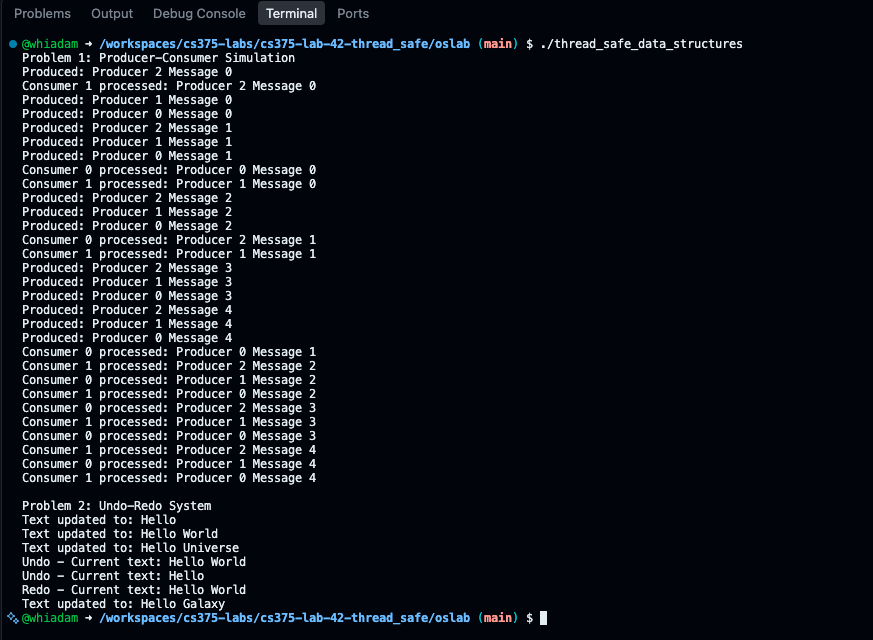
\includegraphics[width=\textwidth]{exercise1_screenshot.png}

\section{Exercise 3: Thread-Safe Priority Queue}
\lstinputlisting[language=C++]{priority_queue.cpp}

This uses std::priority\_queue which keeps the biggest number on top. The mutex makes sure only one thread changes it at a time. 4 threads push 5 random numbers and one thread pops 20 times. The first few pops (88, 91, 90) were just the biggest thing in the queue at that time. After the pushers finished it popped from high to low, 78, 76, 75 down to 0, so the ordering works. 0 items were left at the end.

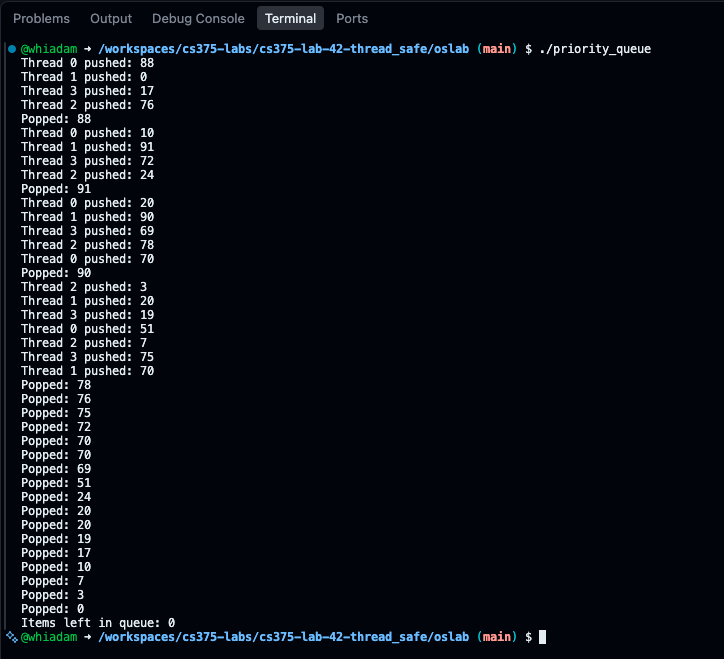
\includegraphics[width=\textwidth]{exercise3_screenshot.png}

\section{Exercise 4: Thread-Safe Circular Buffer}
\lstinputlisting[language=C++]{circular_buffer.cpp}

The buffer is size 5 and in/out wrap around with \%. Push waits on not\_full if the buffer is full and pop waits on not\_empty if its empty, then they notify each other. It has to use unique\_lock because wait needs to unlock and relock. I used 2 producers and 2 consumers like the assignment said. The buffer was empty at the end so everything got consumed.

Compared to the queue in exercise 1, this one has a max size so it cant keep growing, and the threads actually wait instead of just trying again later.

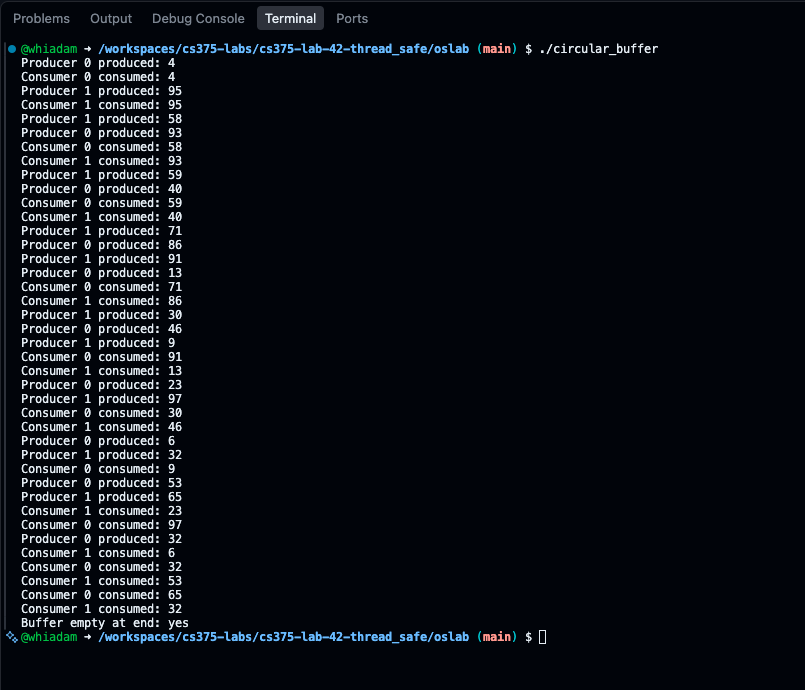
\includegraphics[width=\textwidth]{exercise4_screenshot.png}

\section{Exercise 5: Thread-Safe Deque}
\lstinputlisting[language=C++]{thread_safe_deque.cpp}

I just used one mutex for the whole deque. Front and back can be the same item when there is only 1 thing in it so using separate locks could cause problems. Final size was 0 so nothing got lost. The line ``Popped back: Popped front: 201101'' is because two threads printed at the same time (201 and 101), cout isnt locked so the text got mixed but the data was fine.

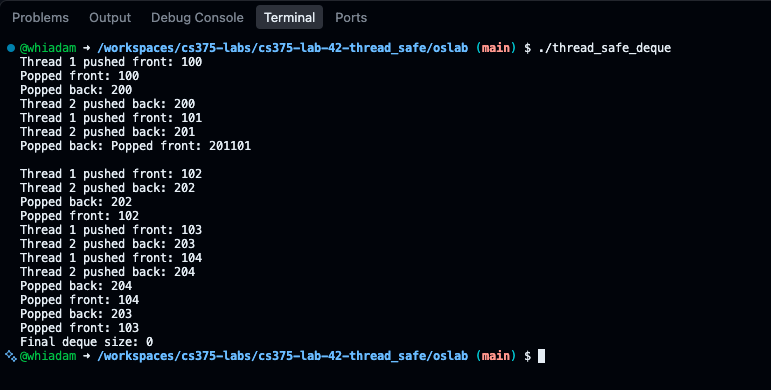
\includegraphics[width=\textwidth]{exercise5_screenshot.png}

\section{Exercise 6: Thread-Safe Linked List}
\lstinputlisting[language=C++]{thread_safe_linked_list.cpp}

Push and pop change head in a few steps so if two threads did it at once a node could get lost or deleted twice. Locking the whole function fixes that. It works like a stack since its all at the front, the last pops were 104, 204, 103, 203, 202, 201, 100. 0 nodes left at the end. The ``Thread Thread 21 pushed'' line is the same printing thing as exercise 5. One lock for the whole list is slower but simpler, size() is the slowest since it goes through every node while locked.

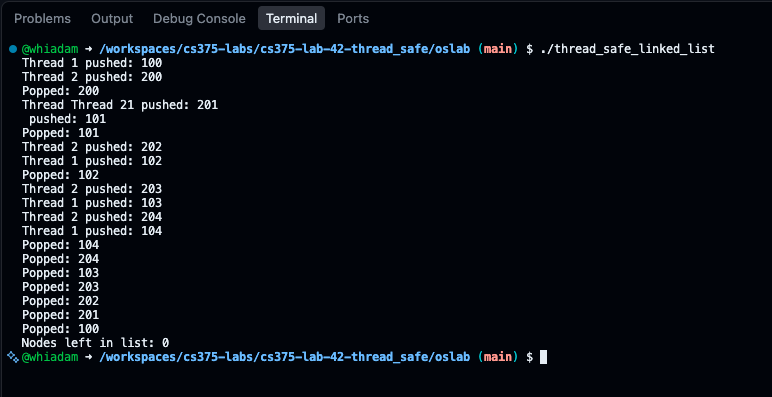
\includegraphics[width=\textwidth]{exercise6_screenshot.png}

\section{Conclusion}
All of them worked and no data was lost. The main thing is that the lock has to cover the whole operation, and cout can get mixed up too if its not locked.

\end{document}
